% !TEX root = paper.tex
% !TEX encoding = UTF-8 Unicode
% -*- coding: UTF-8; -*-
% vim: set fenc=utf-8
% !TEX spellcheck = en-US
\section{Introduction}
\label{sec:intro}
\if 0\CNS
\subsection{Problem statement}
\fi
The prominence of automatic methods to identify objects in natural images is ever increasing. Recently, the performance of such systems outreached the performance of human observers~\citep{He15}. Moreover, these systems which were initially trained on energy greedy, high performance computers are now designed to work on more common hardware such as desktop computers with a decent GPU. \if 0\CNS
However, such methods are not yet available for mobile devices, as will be necessary for instance for the fast detection of visual objects in autonomous driving, as when one has to distinguish a pedestrian from a sign pole. More importantly, the robustness of such methods is still lower than that of humans. Indeed, it is still difficult for such a system to learn to categorize a particular object class given all the possible spatial configurations and the respective geometrical visual transformations. This explosion of combinations is currently handled by increasing accordingly the number of parameters, hence the energy consumption of such methods. As a consequence, state-of-the art classification architectures contain many millions parameters while still handling relatively small images.

\fi On the contrary, the human visual system is able to perform such a feat very rapidly, in less than 100 ms~\citep{Kirchner06}, and at a low energy cost ($<5~W$). On top of that, this system is mostly autonomous, robust to visual transforms or lighting conditions and can learn with a few examples. If many different anatomical features may explain such efficiency, a main difference of the human visual system with classical computer vision approaches in the fact that its sensor (the retina) combines a non homogeneous sampling of the world with the capacity to rapidly change its center of fixation. Indeed, on the one hand, the retina is composed of two separate systems: a central (a disk of about 6 degrees of diameter in visual angle around the center of gaze), high definition fovea and a large, lower definition peripheral area. On the other hand, the retina is attached on the back of the eye which is capable of low latency, high speed eye movements. In particular, saccades allow for efficient changes of the position of the center of gaze: They take about 200 milliseconds to initiate, last about 200 ms and usually reach a maximum velocity of approx 600 degrees per second. This behavior is prevalent during our lifetime (about a saccade every 2-3 seconds, that is, almost a billion saccade in a lifetime). The interplay of those two properties allows to engage observers in an action / perception loop which sequentially scans and analyses the different parts of the image. It is one type of active inference~\citep{Friston12} (see below) and we will envision herein how to incorporate it to classical computer vision schemes.
% (1 / 2.5 * 3600 * 24 * 365 * 75 = 946080000.0 ~= .95e9) X (wakeful + REM = .66)

To explain and take advantage of this visual behavior, it is of particular importance to understand its computational and biological (neurophysiological) principles. One main hypothesis regarding this active vision is that visual scenes most often consist of a single visual object of interest. Take for instance the case of a conversation with a friend at a noisy cafe. To ease the understanding of his voice and emotion you will track his face despite all the remaining sensory clutter by scanning relevant parts of his face with your gaze. Such a visual experience can be simplified in a manner reminiscent to psychophysical experiments: An observer is asked to classify digits (for instance as taken from the MNIST database) as they are shown on a computer display. However, these digits can be placed at a random positions on the display, and visual clutter is added as a background to the image (see Figure~\ref{fig:intro}-A) opening the possibility that the position of this object could be detected in the clutter without being able to identify it before making a saccade to it. This defines more precisely our problem: how do we identify a small object in a large image while not knowing \emph{a priori} its position?

\if 0\CNS
This joint problem of localization and identification is the classical problem of visual search in neuroscience. Such problem is very general and can address complex questions such as "find the green bottle on the table". Here, we will restrict ourselves to a simple "feature search"~\citep{Treisman80}. Such a problem found many solutions in computer vision. Notably, recent advances in deep-learning have provided with efficient models such as faster-RCNN~\citep{Ren17} or YOLO~\citep{Redmon15}. This last implementation is particularly interesting as it predicts in the image the probability of proposed bounding boxes around the visual object. While rapid, the amount of such boxes greatly increases with image size and necessitates a dedicated hardware. When limiting our problem to a few objects of interest in the image, this strategy amounts to a classical problem in neuroscience, that is, the transformation of a luminous image into a saliency map~\citep{Itti01}. Such a computation is essential to understand and predict saccades but also as models of attention. Recently, deep learning methods have extended this type of model by learning to extimate saliency maps over large databases of natural images~\citep{Kummerer16}. While these methods are efficient at predicting the probability of fixation, they miss an essential point in the action perception loop: They operate on the full image while the retina operates on the non-uniform, foveated sampling of visual space (see Figure~\ref{fig:intro}-B). Herein, we believe that this fact is an essential factor to reproduce and understand this active vision process.

An interesting perspective is given with previous modeling of such foveated sensors. The non-uniform sampling of visual space is usually modeled as a log-polar conformal mapping~\citep{Traver10} which has a long history in computer vision and robotics. A first property of this mapping is the separation between the foveal and the peripheral areas as we defined above. This transformation has also other notable properties, such as the correspondence by way of translations in the radial and angular directions to respectively rotations and scalings in the visual domain. However, this sensor is most often not coupled to an action (but see~\citep{ref needed)}. In this paper, we aim at addressing the fragmentation of these different approaches respective to their fields (Machine learning, neuroscience, robotics) to propose an integrated computational model of foveated active vision.
\fi
%------------------------------%
%: see Figure~\ref{fig:intro}
\begin{figure}%[!ht]%%[p!]
%\centering{
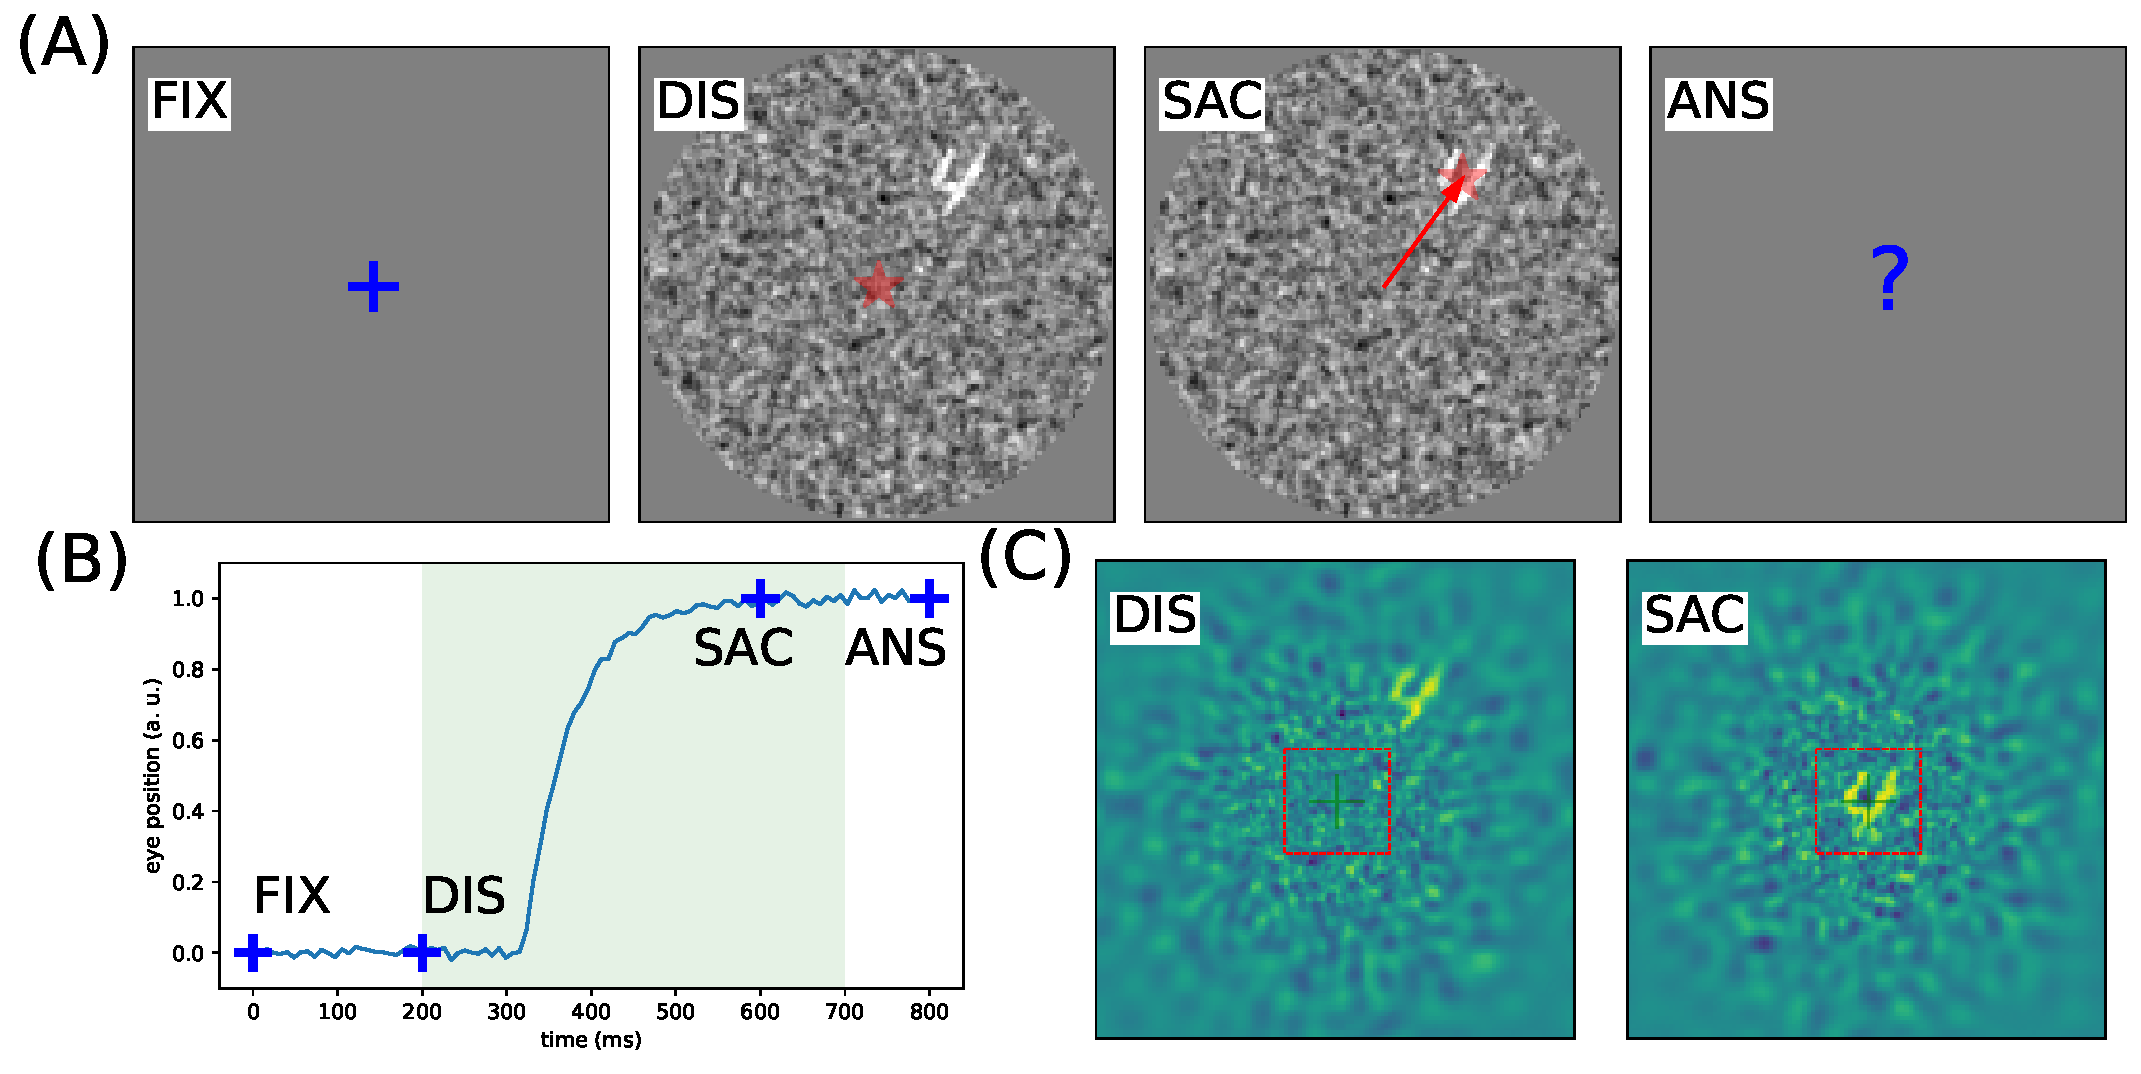
\includegraphics[width=\linewidth]{fig_intro}
%}
\caption{
{\bf Problem setting}: In ecological settings, the visual system is faced to a complex problem when searching for a target and which is synthesized in this thought experiment:
(A)~After a fixation period ('FIX') of $200\ms$, one observer is presented with a luminous display ('DIS') which shows one target from a known class (here digits) and at a random position. The display is presented for a short period but enough to perform one saccade on the potential target ('SAC'). \if 0\CNS In particular, the configuration of the display is such that by adding clutter and reducing the size of the digit it may become necessary to perform a saccade to be able to identify the digit. Finally, the observer identifies the digit ('ANS'). \fi %
(B)~We show a prototypical trace of a saccadic eye movement to the target position.\if 0\CNS In particular, we show the fixation window used to ensure fixation during that window (green shaded area). \fi (C)~These panels show a simulation of the reconstruction from the retinotopic map at respectively ('DIS') the onset of the display and ('SAC') after a (here, successful) saccade. This demonstrates that the position of the target has to be inferred from a degraded (sampled) image ('DIS') and that a correct identification is mediated by the action to the location of the target \emph{before seeing it}, that is before being able to actually be able to identify the target.
\label{fig:intro}}%
\end{figure}%
%%------------------------------%
\if 0\CNS

\subsection{State of the art}
Several studies are relevant to our endeavor. First, one can consider optimal strategies to solve the problem of the visual search of a target~\citep{Najemnik05}. In a setting similar to that presented in Figure~\ref{fig:intro}-A, where the target is an oriented edge and the background is defined as pink noise, authors show first that a Bayesian ideal observer provides with an optimal strategy, and second that human observers are close to that optimal performance. Though they can predict a sequence of saccades in this perception action loop, this model is limited by the simplicity of the display (elementary edges added on stationary noise and a finite number of locations on a discrete grid) and by the abstract level of modeling. Despite these (inevitable) simplifications, this study could successfully predict some key characteristics of visual scanning such as the trade-off between memory content and rapidity.

Looking more closely at neurophysiology, the study of~\citep{Samonds18} allows to go further in our understanding of the interplay between saccadic behavior and the statistics of the input. In this study, authors were able to manipulate the size of saccades by manipulating key properties of the presented (natural) images. For instance, smaller images generate smaller saccades. Interestingly, they also explained the size of saccades for different species, including mice which lack a foveal region, by the size of visual receptive fields. One key prediction of this study which is relevant for our problem is the fact that saccades seem optimal to \emph{a priori} decorrelate the visual input, that is, to minimize redundancy in the sequence of generated saccades, knowing the statistics of visual inputs.

A further modeling perspective is provided by~\citep{Friston12}. In this model, we first have a full description of the visual world as a generative process, here of the presentation of faces, knowing they are constituted of independent components: mouth, nose, eyes, etc... An agent is completely described by giving the generative model governing the dynamics of its internal beliefs and is interacting with this image by scanning it through a foveated sensor, just as we described in Figure~\ref{fig:intro}. Equipping the agent with the ability to actively sample the visual world enables to explore the idea that actions (saccadic eye movements) are optimal experiments, by which the agent seeks to confirm predictive models of the (hidden) world. One key ingredient to this process is the (internal) representation of counterfactual predictions, that is, of the probable consequences of possible hypothesis as they would be realized into actions (here, saccades).

Such a model constitutes an Active Inference scheme~\citep{Mirza18} and simulations of the resulting optimization scheme reproduce sequential eye movements which fit well with empirical data. Compared to~\citet{Najemnik05}, saccades are not the output of a value-based cost function but a consequence of the seek for the agent to minimize the uncertainty about his beliefs, knowing his priors on the generative model of the visual world. Such an approach applies well to our setting, as described in Figure~\ref{fig:intro}. In particular, we will similarly include a generative process of the visual world as image of a handwritten random digit (drawn from the MNIST database) at a random position and embedded in a cluttered noise. Then, we will equip the agent with a foveated sensor and with the ability to actively scan the visual image as defined by a generative (internal) model. Knowing such priors, we will optimize the behavior of this agent and explore its key properties.

\subsection{Outline}
\fi
The goal of this work is to emulate a model of active vision which is able to find a visual target from a known target class, while the position is unknown. This comes with the constraint that the visual sensor is foveated. We will use this constraint as an asset to minimize the overall computational cost of finding the target. This generic visual search problem is of broad general interest in machine learning, computer vision and robotics, but also to neuroscience, as it speaks to the mechanisms underlying foveation and more generally to low-level attention mechanisms. \if 0\CNS

\fi Our aim is to produce a generic principled model and to implement a fast computer implementation thereof. As such, we will start as in~\citep{Friston12} by a probabilistic formulation and use the fundamental hypothesis outlined in Figure~\ref{fig:intro}: The position of an object is independent from its identity. This property is strictly true in our setting and is very generic in vision for simple classes (such as digits) and simple displays\if 0\CNS (but see~\citep{Vo12} for more complex visual scene grammars)\fi . From this independence hypothesis, we may separate the two inter-related tasks (identification vs localization) in two separate pathways with different morphologies (respectively foveal and peripheral). Note that from the retinotopic projection of the visual information, this independence is conditional on action: These pathways should update their beliefs upon decisions made in each respective pathway.

\if 0\CNS
This paper is organized as follows. After this introduction, we will define the notations, variables and equations for the generative process governing the experiment and the generative model for the active vision agent. In particular, we will derive our method to simplify the learning of an optimal agent given these definitions. In section~\ref{sec:results}, we will then show results of numerical simulations of this agent. We will first demonstrate some applications of this framework to different levels of complexity of the problem. This will allow us to derive some limits of this agent and, as in~\citep{Najemnik05}, we will draw some analogies with biologically observed eye movements. Finally, in section~\ref{sec:discussion}, we will summarize these results in comparison with other similar schemes. We will conclude by showing the relative advantages of using this active inference approach.
\fi